\section{Results}
\label{sec:results}

\subsection{Experiment 1: Cross-Model Hallucination Rates}
\label{sec:results_exp1}

\Tabref{tab:halluc_rates} presents per-model hallucination rates on the full 817-question \truthfulqa benchmark.
\gptfourone achieves the lowest hallucination rate at 8.9\%, followed by \gptfouro at 12.5\%.
Notably, \gptfouromini (24.9\%) hallucinates more frequently than the older \gptthreefive (21.3\%), suggesting that model size matters more than training recency for truthfulness on this benchmark.

\begin{table}[t]
    \centering
    \caption{Per-model hallucination rates on \truthfulqa (817 questions). \gptfourone is the most truthful; \gptfouromini has the highest hallucination rate despite being more recent than \gptthreefive.}
    \begin{tabular}{@{}lccc@{}}
        \toprule
        Model & Truthful & Hallucinated & Rate (\%) \\
        \midrule
        \gptfourone     & 744 & 73  & \textbf{8.9} \\
        \gptfouro       & 715 & 102 & 12.5 \\
        \gptthreefive   & 643 & 174 & 21.3 \\
        \gptfouromini   & 614 & 203 & 24.9 \\
        \bottomrule
    \end{tabular}
    \label{tab:halluc_rates}
\end{table}

\para{Frequency of cross-model hallucination.}
\Tabref{tab:freq_dist} shows how many models hallucinate on each question.
A total of 532 questions (65.1\%) cause no hallucinations in any model, while 285 questions (34.9\%) cause at least one model to fail.
Of these, 27 questions (3.3\%) are \emph{universal hallucinations} that fool all four models, and 82 questions (10.0\%) fool three or more.

\begin{table}[t]
    \centering
    \caption{Distribution of questions by the number of models that hallucinate. 27 questions fool all four models; 82 fool three or more.}
    \begin{tabular}{@{}lcc@{}}
        \toprule
        Models hallucinating & Questions & \% of total \\
        \midrule
        0 (none)    & 532 & 65.1 \\
        1 model     & 127 & 15.5 \\
        2 models    & 76  & 9.3 \\
        3 models    & 55  & 6.7 \\
        4 (all)     & \textbf{27}  & \textbf{3.3} \\
        \bottomrule
    \end{tabular}
    \label{tab:freq_dist}
\end{table}

\para{Category analysis.}
\Figref{fig:category_rates} shows hallucination rates by \truthfulqa category.
The highest rates appear in \emph{Confusion: Other} (2.62 mean models wrong per question), \emph{Distraction} (2.14), and \emph{Confusion: People} (1.91).
These categories involve questions where the ``obvious'' answer contradicts the literal truth---precisely the conditions that produce natural hallucinations.

\begin{figure}[t]
    \centering
    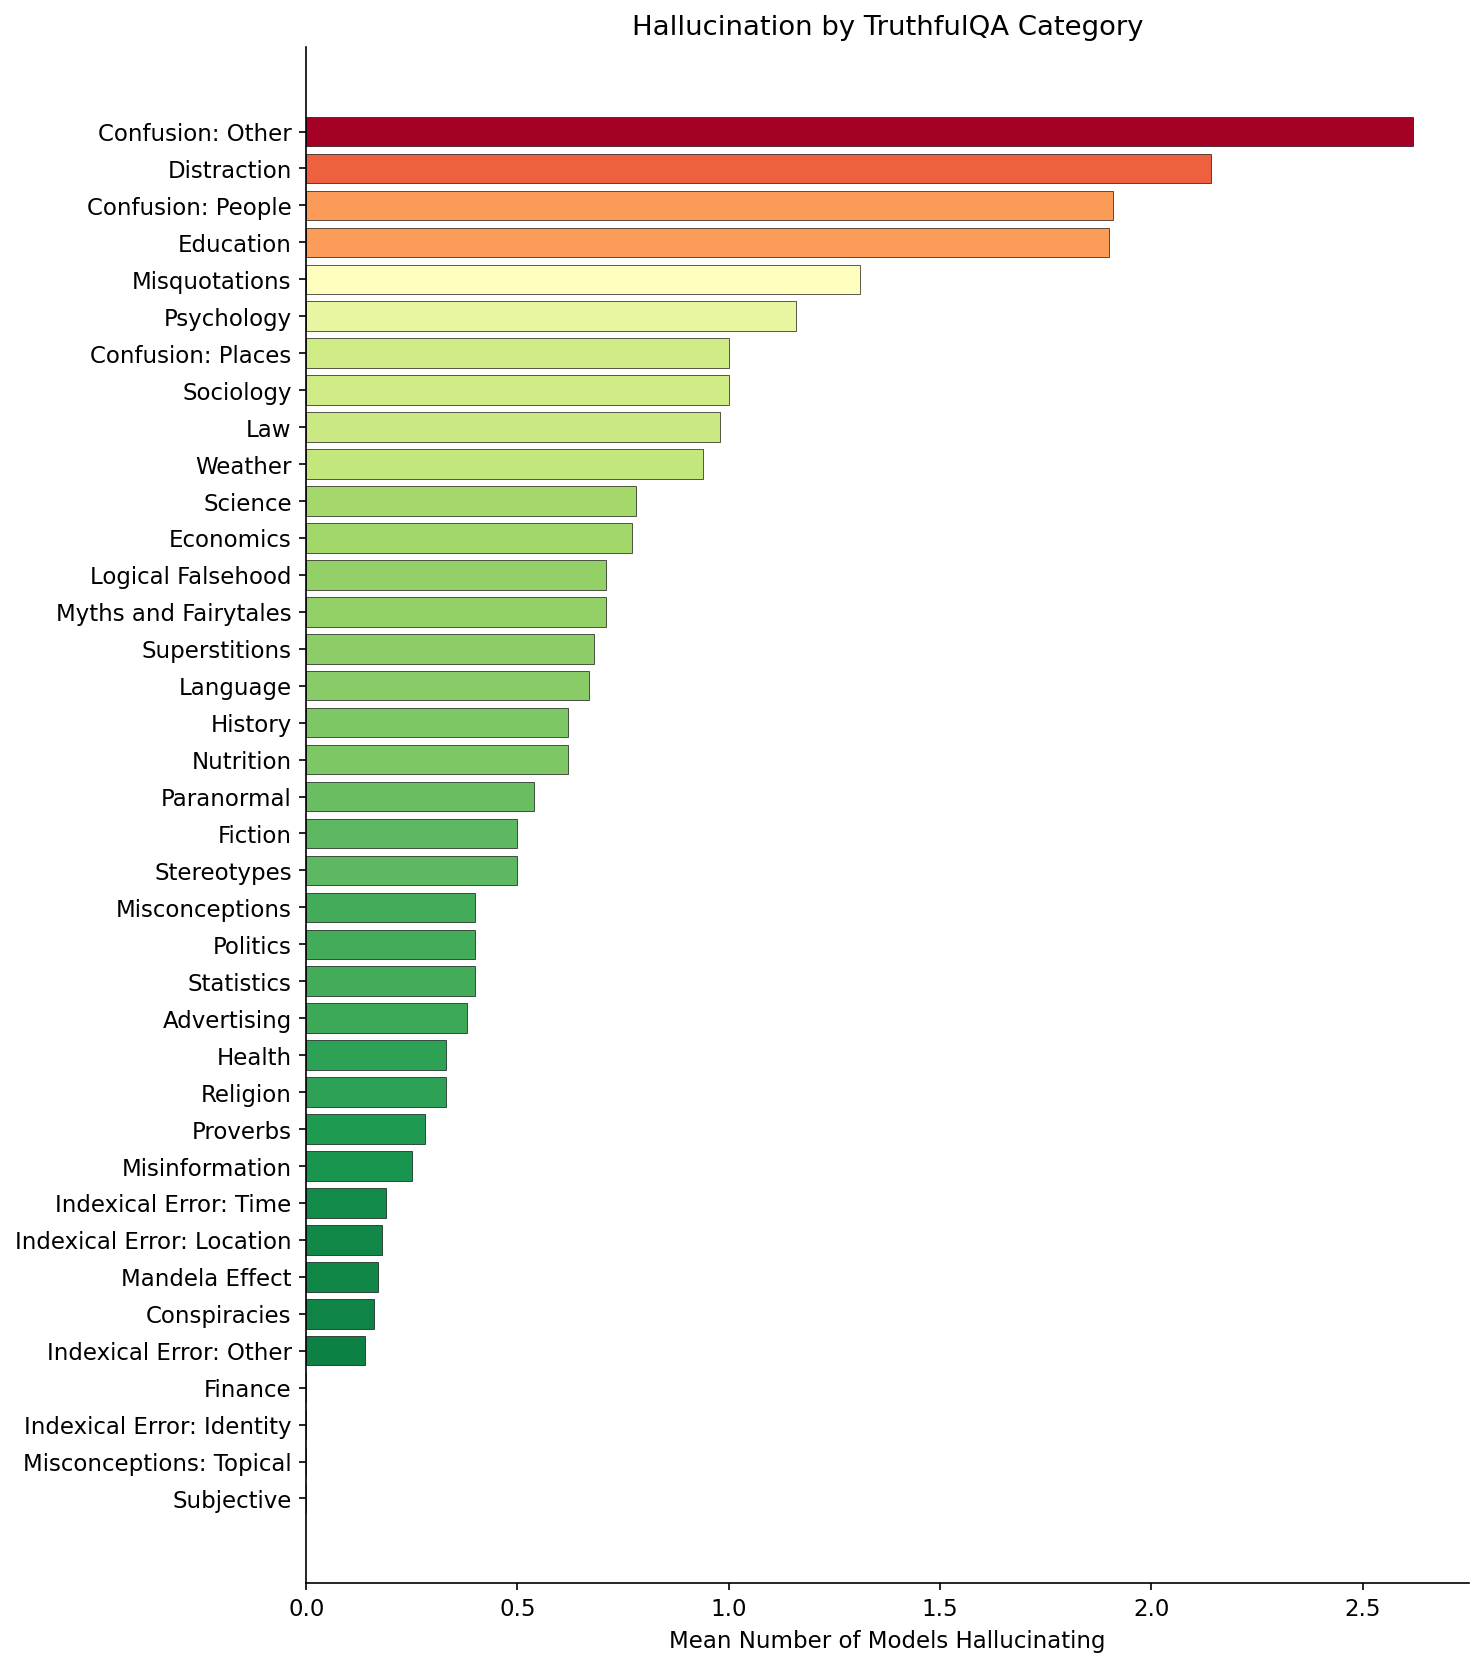
\includegraphics[width=0.95\linewidth]{figures/exp1_category_rates.png}
    \caption{Average number of models hallucinating per question, by \truthfulqa category. Categories involving confusion and distraction show the highest rates, consistent with the natural hallucination hypothesis: errors are worst where common beliefs most strongly contradict the truth.}
    \label{fig:category_rates}
\end{figure}

\subsection{Experiment 2: Robustness to Rephrasing}
\label{sec:results_exp2}

\Tabref{tab:persistence} reports hallucination persistence rates across five rephrasings per question for the 80 selected questions.
The overall mean persistence rate is 76.1\% ($\sigma = 27.8\%$), indicating that the vast majority of hallucinations survive surface-level question variation.

\begin{table}[t]
    \centering
    \caption{Hallucination persistence across five rephrasings. Overall, 76\% of hallucinations survive rephrasing. \gptfouromini shows the highest persistence (85.8\%), suggesting its errors are the most deeply embedded.}
    \begin{tabular}{@{}lcc@{}}
        \toprule
        Model & $N$ hallucinated & Mean persistence (\%) \\
        \midrule
        \gptfouromini   & 76 & \textbf{85.8} \\
        \gptthreefive   & 69 & 75.1 \\
        \gptfourone     & 48 & 72.9 \\
        \gptfouro       & 74 & 69.2 \\
        \midrule
        Overall         & 267 & 76.1 {\scriptsize $\pm$ 27.8} \\
        \bottomrule
    \end{tabular}
    \label{tab:persistence}
\end{table}

\gptfouromini exhibits the highest persistence at 85.8\%, while \gptfouro shows the lowest at 69.2\%.
\Figref{fig:persistence} visualizes the distribution.
These results support hypothesis H1: hallucinations identified by our cross-model survey are not superficial pattern matches triggered by specific phrasings, but reflect deeply embedded incorrect associations.

\begin{figure}[t]
    \centering
    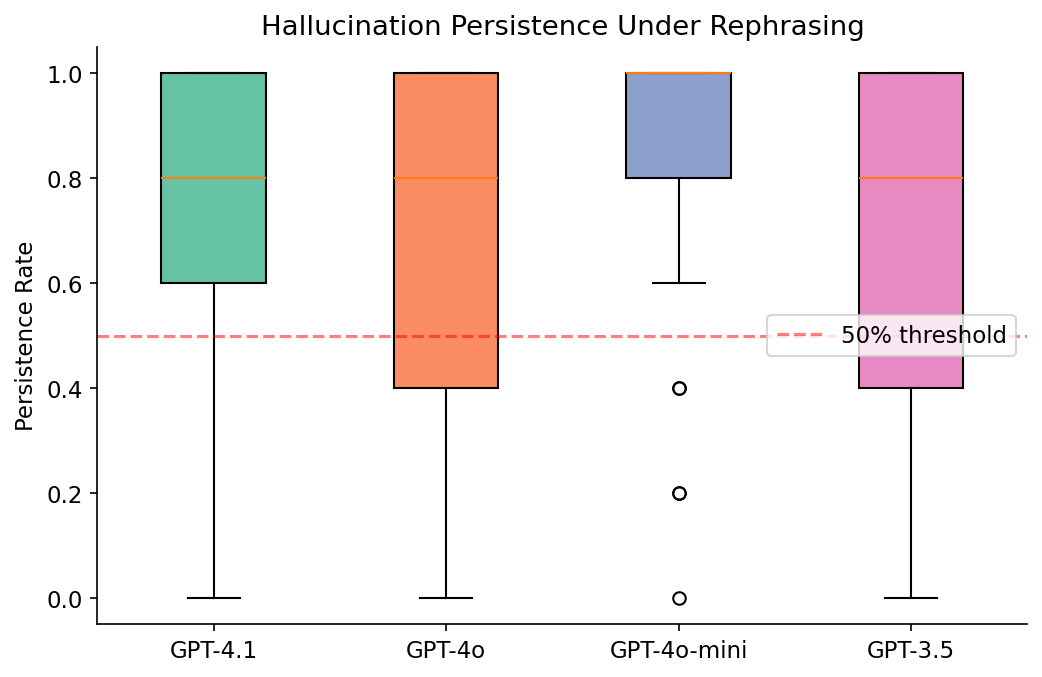
\includegraphics[width=0.75\linewidth]{figures/exp2_persistence.png}
    \caption{Hallucination persistence rates by model across five question rephrasings. Most hallucinations survive rephrasing, with an overall mean of 76.1\%.}
    \label{fig:persistence}
\end{figure}

\subsection{Experiment 3: Self-Detection with Evidence}
\label{sec:results_exp3}

\Tabref{tab:self_detection} presents the central finding of this paper.
When asked to choose between the correct answer and their own hallucinated answer in a randomized A/B test, models select the correct answer only 10--16\% of the time.
This is not merely below the 66--95\% accuracy they achieve on control questions---it is below the 50\% chance baseline.
The models are \emph{systematically biased toward their own wrong answer}.

\begin{table}[t]
    \centering
    \caption{Self-detection accuracy: models choose between the correct answer and their own hallucinated answer (order randomized). All models perform far below chance (50\%) on hallucinated questions while achieving high accuracy on controls. The gap ranges from 56 to 81 percentage points.}
    \begin{tabular}{@{}lccc@{}}
        \toprule
        Model & Hallucination (\%) & Control (\%) & Gap (pp) \\
        \midrule
        \gptfourone     & 16.4 & 95.0 & 78.6 \\
        \gptfouro       & 13.8 & 95.0 & 81.2 \\
        \gptfouromini   & 10.0 & 87.5 & 77.5 \\
        \gptthreefive   & 10.0 & 66.2 & 56.2 \\
        \bottomrule
    \end{tabular}
    \label{tab:self_detection}
\end{table}

The overall difference is highly significant ($z = 18.49$, $p < 0.0001$, effect size $= 0.735$).
\Figref{fig:self_detection} illustrates the dramatic gap between hallucination and control conditions.
This result strongly supports hypothesis H2 and has important implications for self-verification approaches: if a model cannot distinguish its own error from the truth even when both are presented side by side, output-layer self-critique is unlikely to catch natural hallucinations.

\begin{figure}[t]
    \centering
    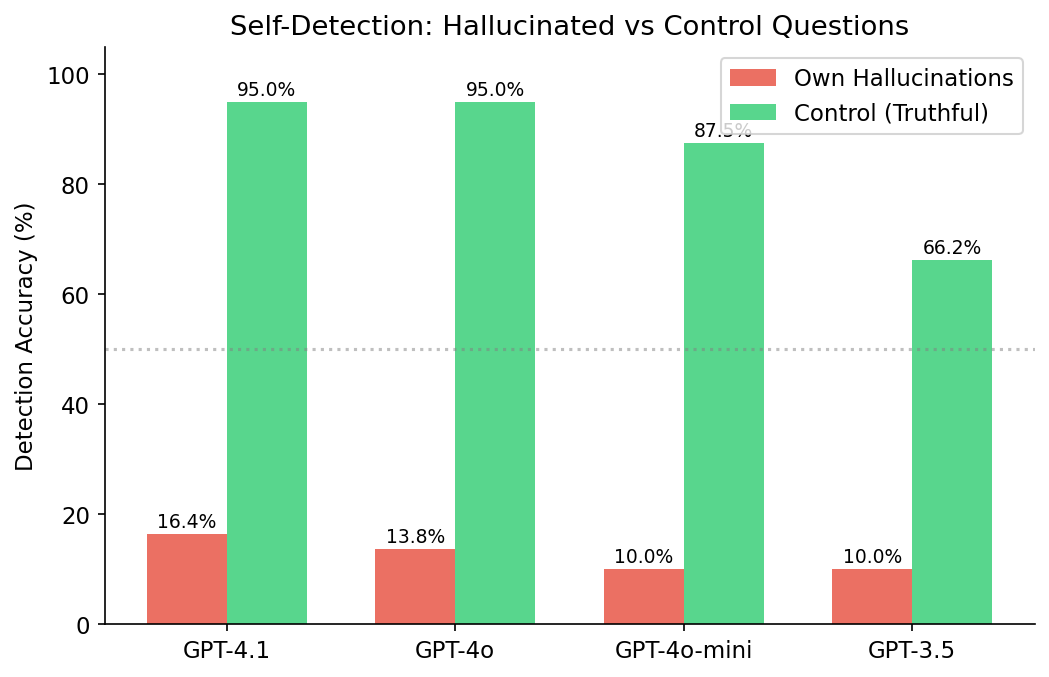
\includegraphics[width=0.75\linewidth]{figures/exp3_self_detection.png}
    \caption{Self-detection accuracy on hallucinated versus control questions. On hallucinated questions, all models perform below 50\% chance (dashed line), indicating systematic bias toward their own incorrect answer. Control accuracy is dramatically higher.}
    \label{fig:self_detection}
\end{figure}

\subsection{Experiment 4: Cross-Model Transfer}
\label{sec:results_exp4}

\para{Pairwise overlap.}
\Tabref{tab:jaccard} reports pairwise Jaccard similarity between models' hallucination sets.
All pairs show overlap 3--6$\times$ above the random baseline computed via permutation testing (1,000 permutations), with all $p < 0.001$.
The highest overlap (0.412) appears between \gptfouromini and \gptthreefive---models of similar capability---while the lowest (0.193) appears between \gptfourone and \gptthreefive, the pair with the largest capability gap.

\begin{table}[t]
    \centering
    \caption{Pairwise Jaccard similarity of hallucination sets. All values are 3--6$\times$ above random baseline (permutation test, 1,000 iterations, all $p < 0.001$). Higher values indicate greater overlap in which specific questions cause hallucinations.}
    \begin{tabular}{@{}llccc@{}}
        \toprule
        Model A & Model B & Jaccard & Random & Ratio \\
        \midrule
        \gptfouromini & \gptthreefive  & \textbf{0.412} & 0.130 & 3.2$\times$ \\
        \gptfouro     & \gptfouromini  & 0.399 & 0.091 & 4.4$\times$ \\
        \gptfourone   & \gptfouro      & 0.357 & 0.056 & \textbf{6.4$\times$} \\
        \gptfouro     & \gptthreefive  & 0.314 & 0.086 & 3.7$\times$ \\
        \gptfourone   & \gptfouromini  & 0.243 & 0.071 & 3.4$\times$ \\
        \gptfourone   & \gptthreefive  & 0.193 & 0.068 & 2.8$\times$ \\
        \bottomrule
    \end{tabular}
    \label{tab:jaccard}
\end{table}

\para{Temporal prediction.}
\Tabref{tab:temporal} shows that older-model hallucinations significantly predict newer-model hallucinations.
If \gptthreefive hallucinated on a question, \gptfourone is 4.5$\times$ more likely to hallucinate on that same question (23.0\% versus 5.1\%).
The effect is even stronger within the GPT-4 family: if \gptfouromini hallucinates, \gptfouro is 18.7$\times$ more likely to hallucinate (42.9\% versus 2.3\%).

\begin{table}[t]
    \centering
    \caption{Temporal prediction of hallucinations. $P(\text{new wrong} \mid \text{old wrong})$ is the probability that the newer model hallucinates given that the older model hallucinated on the same question. Both correlations are highly significant ($p < 0.0001$).}
    \begin{tabular}{@{}lcccc@{}}
        \toprule
        Direction & $r$ & $P(\text{new} \mid \text{old wrong})$ & $P(\text{new} \mid \text{old right})$ & Ratio \\
        \midrule
        \gptthreefive $\to$ \gptfourone & 0.256 & 23.0\% & 5.1\% & 4.5$\times$ \\
        \gptfouromini $\to$ \gptfouro   & \textbf{0.528} & 42.9\% & 2.3\% & \textbf{18.7$\times$} \\
        \bottomrule
    \end{tabular}
    \label{tab:temporal}
\end{table}

\Figref{fig:jaccard_heatmap} visualizes the full pairwise Jaccard matrix.
The pattern is clear: models that hallucinate tend to hallucinate on the \emph{same questions}, and this overlap is far too large to be explained by chance.

\begin{figure}[t]
    \centering
    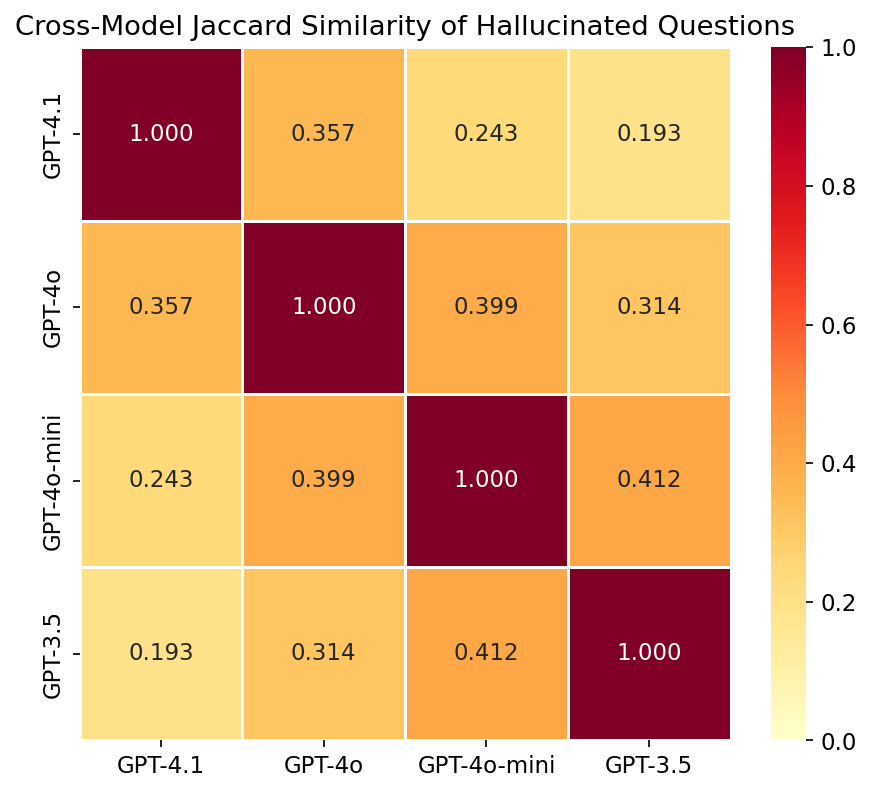
\includegraphics[width=0.65\linewidth]{figures/exp4_jaccard_heatmap.png}
    \caption{Pairwise Jaccard similarity heatmap of hallucination sets across four models. Darker cells indicate higher overlap. All pairwise similarities are significantly above the random baseline ($p < 0.001$).}
    \label{fig:jaccard_heatmap}
\end{figure}
